
\hypertarget{cv:registrarCU}{\section{Registrar Caso de Uso}} \label{sec:registrarCU}

	Esta funcionalidad le permitirá registrar un caso de uso dentro del proyecto que se esta operando.

		\subsection{Procedimiento}

			%Pasos de procedimiento
			\begin{enumerate}
	
			\item Oprima el botón \IURegistrar{} de la pantalla \ref{fig:GestionarCU} ''Gestionar Casos de Uso''.
			
			\item Se mostrará la pantalla \ref{fig:registrarCUA} ''Registrar Caso de Uso''.

			%Pantalla
			\begin{figure}[H]
				\begin{center}
					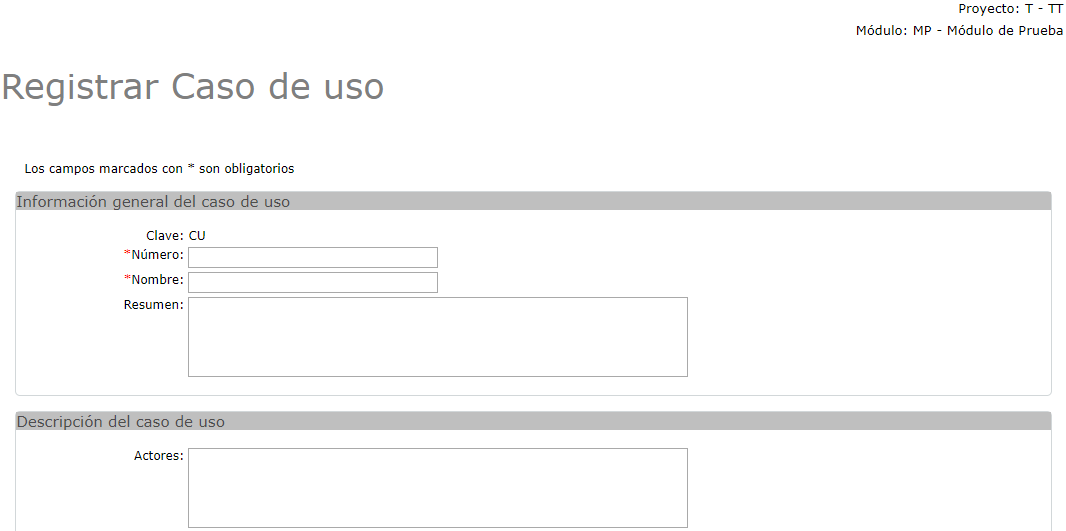
\includegraphics[scale=0.6]{roles/lider/casosUso/pantallas/IU12-1registrarCUA}
					\caption{Registrar Caso de Uso}
					\label{fig:registrarCUA}
				\end{center}
			\end{figure}
		
		%Pantalla
		\begin{figure}[H]
			\begin{center}
				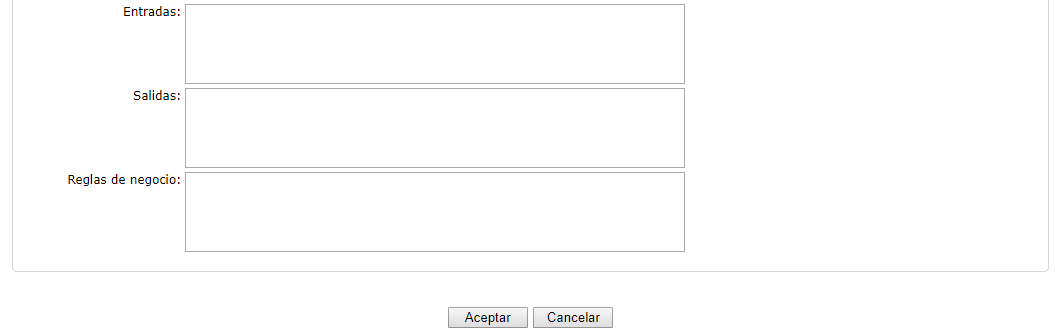
\includegraphics[scale=0.6]{roles/lider/casosUso/pantallas/IU12-1registrarCUB}
				\caption{Registrar Caso de Uso}
				\label{fig:registrarCUB}
			\end{center}
		\end{figure}
		
			\item Ingrese el número, nombre  y el resumen del caso de uso.
			
			\item Para la sección de ''Descripción del caso de uso'' podrá ingresar TOKENS para vincular diferentes elementos previamente registrados dependiendo de cada campo en el que se encuentre:
			
			\begin{itemize}
				\item En el campo de actores solo podrá referenciar elementos de tipo actor con el TOKEN: ''ACT·''.
				\item En el campo de entradas solo podrá referenciar elementos de tipo entidad, atributos y términos de glosario con los TOKEN: ''ENT·'', ''ATR·'' y ''GLS·''.
				\item En el campo de salidas solo podrá referenciar elementos de tipo entidad, atributos y términos de glosario con los TOKEN: ''ENT·'', ''ATR·'', ''GLS·'' y ''MSG·''.
				\item En el campo de reglas de negocio solo podrá referenciar elementos de tipo regla de negocio con el TOKEN: ''RN·''.
			\end{itemize}
			
			\item Oprima el botón \IUAceptar.
			
			\item Se mostrará el mensaje \ref{fig:CURegistrado} en la pantalla \ref{fig:GestionarCU} ''Gestionar Casos de Uso''.
			
			\begin{figure}[htbp!]
				\begin{center}
					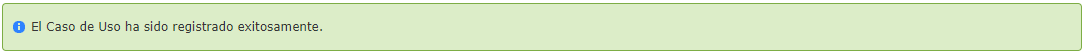
\includegraphics[scale=0.6]{roles/lider/casosUso/pantallas/IU12-1MSG1}
					\caption{MSG: Caso de Uso Registrado}
					\label{fig:CURegistrado}
				\end{center}
			\end{figure}
			\end{enumerate}